\documentclass[10pt,a4paper]{article}
\usepackage[margin=2cm]{geometry}
\usepackage[T1]{fontenc}
\usepackage[utf8]{inputenc}
\usepackage{lmodern}
\usepackage{amsmath,amssymb}
\usepackage{booktabs}
\usepackage{graphicx}
\usepackage{xcolor}
\usepackage{caption}
\usepackage[hidelinks]{hyperref}
\usepackage{enumitem}
\setlist{nosep,leftmargin=*}
\captionsetup{font=small,labelfont=bf}
\setlength{\parskip}{3pt}
\setlength{\parindent}{0pt}

% Placeholder for numbers that are still being computed. Remove before submitting.
\newcommand{\todo}[1]{\textcolor{red}{[TODO: #1]}}
\newcommand{\x}{\mathbf{x}}
\newcommand{\m}{\mathbf{m}}
\newcommand{\dd}{\boldsymbol{\delta}}

\graphicspath{{../results/}}

\title{\vspace{-1.2cm}\textbf{Sparse Adversarial Attacks with Grad-CAM and Learnable Masks}\\[2pt]
\large EE 48012 / 58012 --- Graded Assignment 1}
\author{Ay\c{s}e Nil \"Ozdemir \quad \todo{student ID}\\[2pt]
\small Code: \url{https://github.com/nilozdemir/EE58012}}
\date{}

\begin{document}
\maketitle
\vspace{-0.8cm}

\section{Setup}

\textbf{Model.} The clean model is the CIFAR-variant ResNet-18 of Self-Study 2
(3$\times$3 stride-1 stem, no max-pooling), with input normalisation as its first
layer, so the attack works on images in $[0,1]$ and the normalisation is applied
after $\x'$ is formed. It was trained with SGD (momentum 0.9, lr 0.1, cosine
schedule with one warm-up epoch, weight decay $5\cdot10^{-4}$, batch 128, random
crop and flip) for 100 epochs and reaches \textbf{94.82\%} clean test accuracy.
All 9{,}482 correctly classified test images are attacked; ASRs are fractions of
these images. With $n=9482$ the standard error of an ASR,
$\sqrt{p(1-p)/n}$, is at most about 0.5 percentage points (pp; reached at an ASR of
50\%), so differences below about 1\,pp are not significant.

\textbf{Threat model.} $\x'=\x+\m\odot\dd$, with $\m\in\{0,1\}^{32\times32}$ shared
by the three channels, exactly $k=\rho\cdot1024$ ones ($k=256$ and $512$),
$\|\dd\|_\infty\le\varepsilon=2/255$ and $\x'\in[0,1]^{3\times32\times32}$. The
targeted attack uses $t=(y+1)\bmod 10$. Every returned example is checked against
these constraints in code, and the ASR is computed on a fresh forward pass of the
returned binary-mask examples (no example violated a constraint, and the fresh
evaluation agreed with the success recorded during the attack for every image).

\textbf{Optimisation of $\dd$ (all masks).} For a fixed mask, $\dd$ is found by
signed-gradient PGD with a random start $\dd_0\sim U[-\varepsilon,\varepsilon]$,
100 steps of size $\alpha=2.5\,\varepsilon/100$, and projection onto
$\{\|\dd\|_\infty\le\varepsilon,\ \x+\dd\in[0,1]\}$. The objective is the
cross-entropy of $y$ (maximised, untargeted) or of $t$ (minimised, targeted). Every
iterate is a valid sparse example, so an image counts as a success if any iterate
succeeds. Grad-CAM, random and learned masks all use exactly this procedure.

\section{Part A: Grad-CAM as a sparsity mask}

\subsection{Method}

\textbf{Layer.} With the CIFAR stem the stages of ResNet-18 output
\texttt{layer1} $64\times32\times32$, \texttt{layer2} $128\times16\times16$,
\texttt{layer3} $256\times8\times8$ and \texttt{layer4} $512\times4\times4$. We use
\textbf{\texttt{layer3} (256$\times$8$\times$8)}: an $8\times8$ map has four times as
many cells as \texttt{layer4}, so a mask of 256 or 512 pixels can follow its shape,
while the features are still high-level enough to be class-specific.

\textbf{Map.} For a score $S(\x)$ (a logit or a difference of logits, never a
softmax probability), Grad-CAM gives
$L_S=\sum_c\alpha_c A^c$ with $\alpha_c=\frac{1}{64}\sum_{ij}\partial S/\partial A^c_{ij}$,
where $A$ is the output of \texttt{layer3}. The map is bilinearly upsampled to
$32\times32$.

\textbf{From map to mask.} The mask is the top-$k$ of the upsampled map. We rank the
map \emph{before} the ReLU of Grad-CAM: the ReLU does not change the order of the
positive locations, but often fewer than $k$ locations are positive (especially for
the targeted maps, Fig.~\ref{fig:gradcam}), and the pre-ReLU values still rank the
remaining pixels instead of breaking ties arbitrarily.

\textbf{Score per attack.}
\begin{itemize}
\item \emph{Untargeted:} $S=z_y$, the true-class logit. Its map marks where the
evidence for $y$ lies; perturbing these pixels should remove that evidence.
\item \emph{Targeted:} $S=z_t-z_y$, the margin the attack has to make positive. Its
channel weights are $\nabla z_t-\nabla z_y$, so the map marks locations whose
features both add evidence for $t$ and take it away from $y$. This was our
\emph{a priori} choice; Section~\ref{sec:ablation} compares it with the maps of $z_y$
and $z_t$.
\end{itemize}
The random baseline draws $k$ pixels uniformly at random per image (top-$k$ of
i.i.d.\ uniform scores, seed 0).

Fig.~\ref{fig:gradcam} shows the maps and masks for the first five correctly
classified test images.

\begin{figure}[t]
\centering
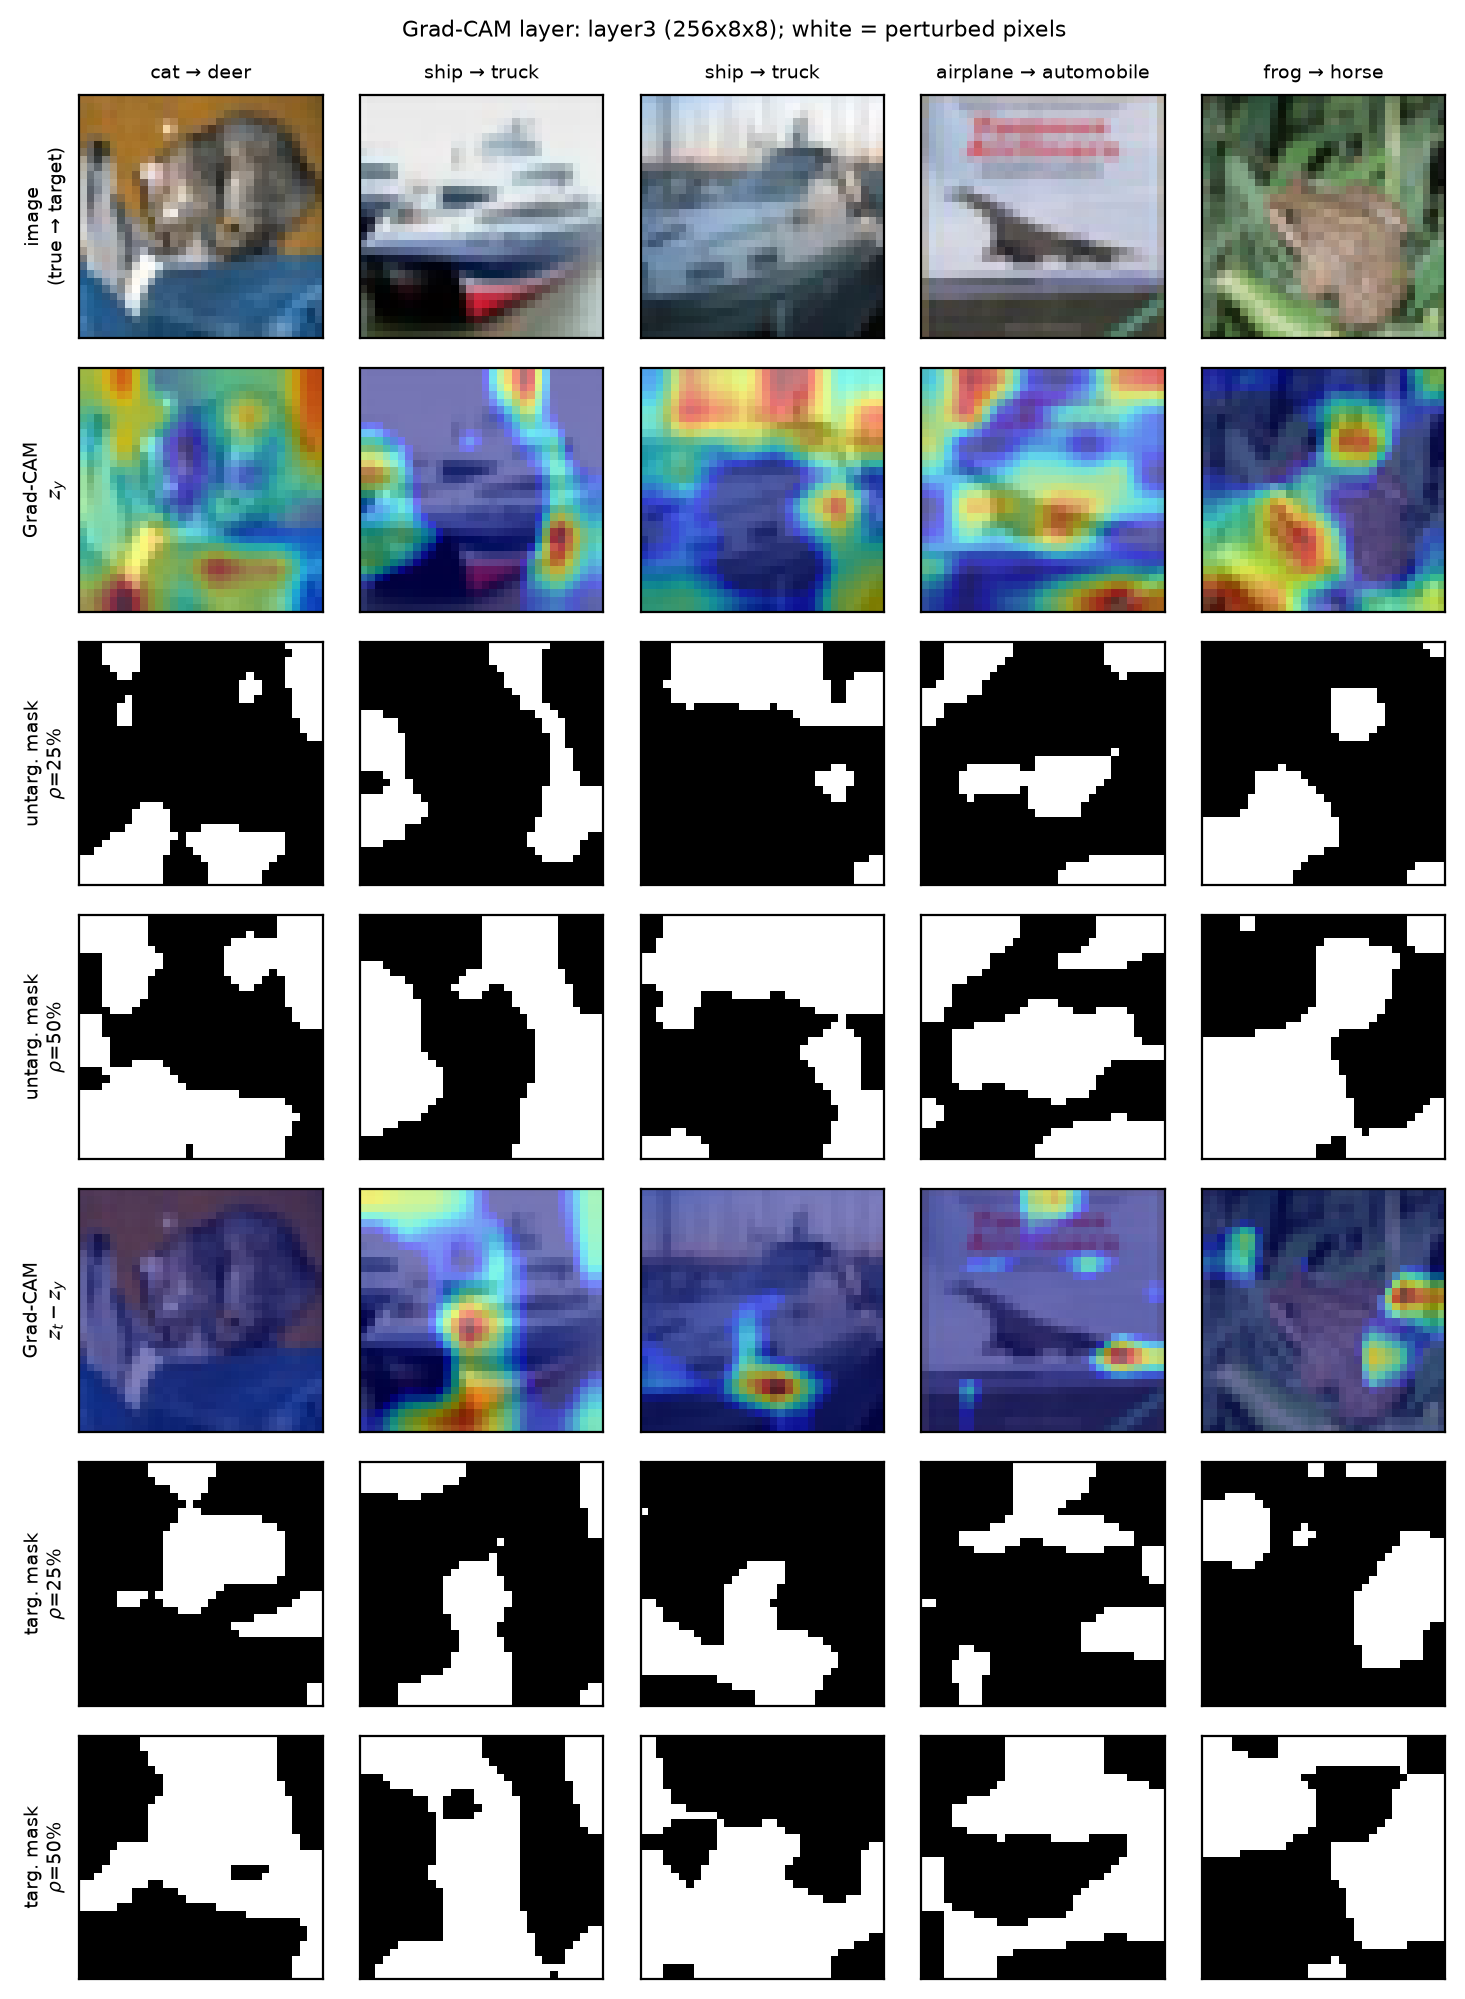
\includegraphics[width=0.66\linewidth]{fig_gradcam_masks.png}
\caption{Grad-CAM at \texttt{layer3} ($8\times8$, upsampled) and the resulting
masks for five test images (title: true $\to$ target class). Row 2: map of $z_y$
(untargeted); rows 3--4: its top-$k$ masks for $\rho=25\%$ and $50\%$. Row 5: map
of $z_t-z_y$ (targeted); rows 6--7: its masks. Heatmaps are shown after the ReLU and
normalised to $[0,1]$; the masks are ranked on the pre-ReLU maps. White = perturbed
pixels.}
\label{fig:gradcam}
\end{figure}

\subsection{Evaluation}

\begin{table}[t]
\centering
\caption{ASR (\%) over the 9{,}482 correctly classified test images,
$\varepsilon=2/255$. Parts A and B use the same PGD for $\dd$ (100 steps); the
learned masks additionally run 100 joint mask--$\dd$ steps (Section~\ref{sec:b}).
The last two rows are a control: Part A with 200 PGD steps.}
\label{tab:asr}
\begin{tabular}{lcccc}
\toprule
& \multicolumn{2}{c}{untargeted} & \multicolumn{2}{c}{targeted} \\
\cmidrule(lr){2-3}\cmidrule(lr){4-5}
Mask & $\rho=25\%$ & $\rho=50\%$ & $\rho=25\%$ & $\rho=50\%$ \\
\midrule
Grad-CAM mask (A) & 30.6 & 58.8 & 6.3 & 25.2 \\
Random mask (A) & 24.6 & 57.3 & 6.2 & 27.0 \\
\midrule
Learned, Grad-CAM init (B) & \textbf{36.2} & \textbf{69.8} & \textbf{12.3} & 42.9 \\
Learned, random init (B) & 31.9 & 69.2 & 11.7 & \textbf{43.9} \\
\midrule
\multicolumn{5}{l}{\emph{Control: Part A with 200 PGD steps}}\\
Grad-CAM mask & 30.6 & 58.9 & 6.4 & 25.4 \\
Random mask & 24.6 & 57.5 & 6.2 & 27.1 \\
\bottomrule
\end{tabular}
\end{table}

\begin{table}[t]
\centering
\caption{Targeted attack: which Grad-CAM score is used to rank the pixels
(same PGD as Table~\ref{tab:asr}). ASR in \%.}
\label{tab:ablation}
\begin{tabular}{lcc}
\toprule
Mask (targeted, $t=(y+1)\bmod10$) & $\rho=25\%$ & $\rho=50\%$ \\
\midrule
Grad-CAM of $z_t-z_y$ (margin; used in Table~\ref{tab:asr}) & 6.3 & 25.2 \\
Grad-CAM of $z_t$ (target logit) & 8.0 & 28.0 \\
Grad-CAM of $z_y$ (true logit) & \textbf{8.7} & \textbf{29.7} \\
Random mask & 6.2 & 27.0 \\
\bottomrule
\end{tabular}
\end{table}

Table~\ref{tab:asr} (top) gives the ASR of the Grad-CAM and random masks, and
Table~\ref{tab:ablation} compares three ways of using Grad-CAM for the targeted
mask. Doubling the PGD steps to 200 changes the Part A ASRs by at most 0.2\,pp
(Table~\ref{tab:asr}, bottom), so 100 steps have converged and the
comparison is not limited by the optimisation of $\dd$.

\subsection{Questions}
\label{sec:ablation}

\textbf{Does Grad-CAM help compared with a random mask?} For the untargeted attack,
yes, and most clearly when the budget is tight: $+6.0$\,pp at $\rho=25\%$
(30.6 vs.\ 24.6\%, a relative gain of 24\%) but only $+1.5$\,pp at $\rho=50\%$.
For the targeted attack our \emph{a priori} margin mask does not help (6.3 vs.\
6.2\% at 25\%, and 25.2 vs.\ 27.0\% at 50\%). Grad-CAM of the true class does help
for the targeted attack too (8.7 and 29.7\%, i.e.\ $+2.5$ and $+2.7$\,pp over random,
Table~\ref{tab:ablation}). The gains are modest in all cases: an $8\times8$ map
upsampled to $32\times32$ selects large blobs, and the maps of $z_y$ often highlight
background or object edges rather than the object itself (Fig.~\ref{fig:gradcam},
cat and first ship), so Grad-CAM indicates roughly \emph{where} the model looks
but not which individual pixels are most sensitive.

\textbf{Why did we use Grad-CAM differently for the targeted attack?} The targeted
attack must both lower $z_y$ and raise $z_t$, so we expected the map of the margin
$z_t-z_y$, which combines both gradients, to be the right one. Table~\ref{tab:ablation}
shows the opposite ordering: $z_y$ (8.7\%) $>$ $z_t$ (8.0\%) $>$ random (6.2\%)
$\approx$ margin (6.3\%) at $\rho=25\%$, and the same at $50\%$. Two effects explain
this. (i) The margin map is very concentrated: in Fig.~\ref{fig:gradcam} (row 5) at most one
or two hot spots are positive, and for the cat none, so a mask of 256 or 512
pixels is mostly filled by ranking negative, low-magnitude values, which carry
little information; the masks then become fragmented (rows 6--7). (ii) For a
correctly classified image, $z_y$ is far above $z_t$, and the most effective way to
close the gap is to destroy the evidence for $y$, which is spread over the object;
the evidence for $t$ that can be created with $\varepsilon=2/255$ is small. Hence
the best targeted mask uses Grad-CAM \emph{in the same way} as the untargeted one
(map of $z_y$). We keep the margin mask in Table~\ref{tab:asr} because it was the
method fixed before the experiment, and report the better variant here.

\textbf{How does the ASR change from 25\% to 50\%?} It rises steeply: about
$\times2$ for the untargeted attack (30.6 $\to$ 58.8\% with Grad-CAM, 24.6 $\to$
57.3\% random) and about $\times4$ for the targeted one (6.3 $\to$ 25.2\%, 6.2
$\to$ 27.0\%). With $\varepsilon=2/255$ the attack is very weak per pixel, so its
strength grows with the number of perturbed pixels: to first order the change of
the loss is bounded by $\varepsilon\sum_{ij}m_{ij}\sum_c|\partial L/\partial x_{cij}|$,
which roughly doubles with $k$. The targeted attack needs a larger change (it must
reach one specific class), so it benefits more. At the same time the advantage of
Grad-CAM over random shrinks (6.0 $\to$ 1.5\,pp untargeted): with half of the
image perturbed, the two masks overlap in about half their pixels in expectation,
and choosing \emph{which} pixels matters less.

\section{Part B: Learnable mask}
\label{sec:b}

\subsection{Method}

Each image gets a real score $s_{ij}$ per pixel, and the mask is always its top-$k$
projection, $\m=\mathrm{TopK}(\mathbf{s},k)$. The mask is therefore binary with
exactly $k$ ones at \emph{every} step, so there is no gap between a continuous mask
used during optimisation and the final binary mask, and every iterate is a valid
sparse example. Top-$k$ has zero gradient almost everywhere, so $\mathbf{s}$ is trained
with a straight-through estimator that treats $\m$ as if it were $\mathbf{s}$ in the
backward pass:
\[
\frac{\partial L}{\partial s_{ij}} := \frac{\partial L}{\partial m_{ij}}
= \sum_{c}\delta_{cij}\,\frac{\partial L}{\partial x'_{cij}},
\]
the first-order change of the attack objective $L$ when pixel $(i,j)$ is switched
on with its current perturbation. To make this signal meaningful for pixels that are
currently off, $\dd$ is kept on \emph{all} pixels and updated with the unmasked
gradient at $\x'$, so a pixel that enters the mask brings the perturbation it would
have had. Per batch of images:
\begin{enumerate}
\item Initialise $\mathbf{s}$ from the Grad-CAM map of Part A (standardised to zero
mean and unit variance per image) or from i.i.d.\ uniform noise (also standardised);
$\dd\sim U[-\varepsilon,\varepsilon]$.
\item Repeat 100 times: $\m=\mathrm{TopK}(\mathbf{s},k)$, $\x'=\x+\m\odot\dd$,
$\mathbf{g}=\nabla_{\x'}L$;\;
$\dd\leftarrow\Pi(\dd+\alpha\,\mathrm{sign}(\mathbf{g}))$ on all pixels;\;
one Adam step (lr 0.05) on $\mathbf{s}$ in the direction that increases $L$.
\item Fix the final binary mask $\m=\mathrm{TopK}(\mathbf{s},k)$ and finish $\dd$ with
the same 100-step PGD as Part A, starting from the current $\dd$.
\end{enumerate}
An image is a success if any iterate of step 2 or 3 succeeds; the returned example,
its mask and the reported ASR use only binary masks with $k$ pixels. The two
initialisations use identical settings (same $\alpha$, steps, learning rate and
seed). Because the learned mask uses 100 joint steps on top of the 100 PGD steps of
Part A, Table~\ref{tab:asr} also reports Part A with 200 PGD steps as a control.

\subsection{Evaluation}

Table~\ref{tab:asr} (middle) reports the learned masks next to the Grad-CAM mask of
Part A. Each configuration took about 85\,s on a single GPU for 9{,}482 images,
twice the cost of Part A.

\begin{figure}[t]
\centering
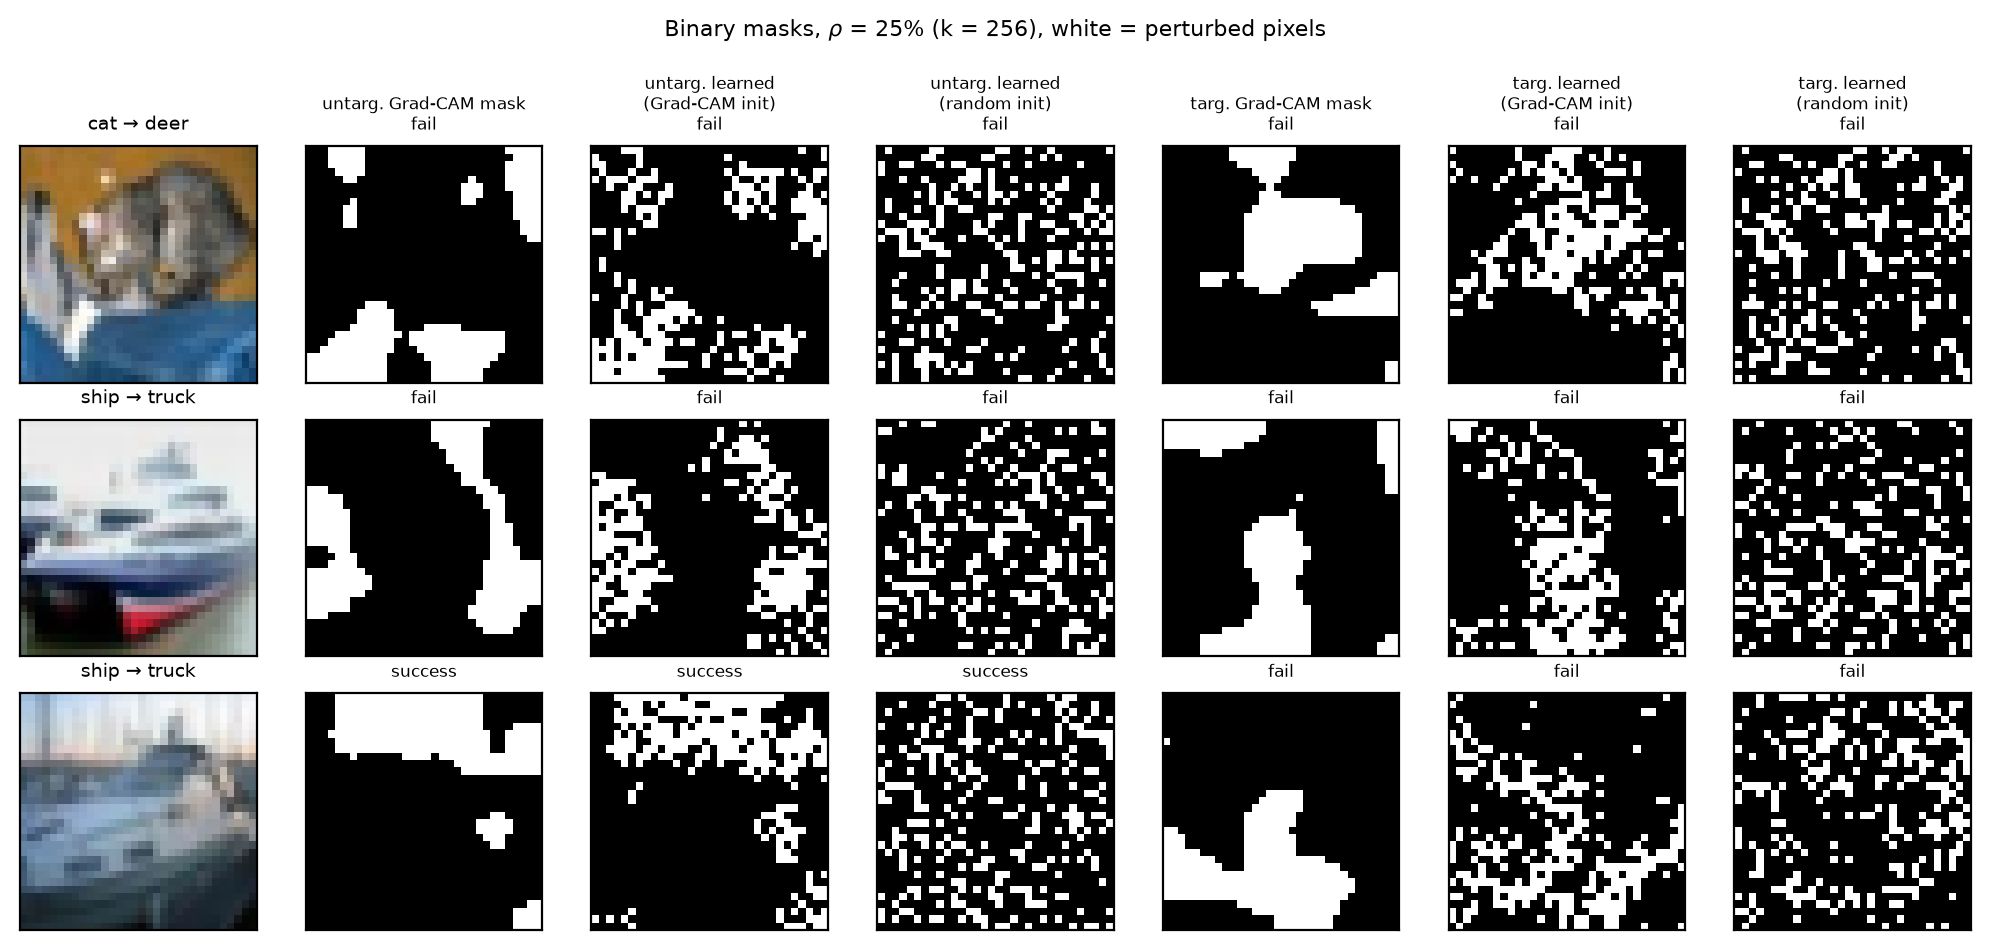
\includegraphics[width=\linewidth]{fig_learned_vs_gradcam.png}
\caption{Grad-CAM mask (Part A) and learned masks (Part B, Grad-CAM and random
initialisation) side by side for the first three test images, $\rho=25\%$, for the
untargeted (columns 2--4) and targeted (columns 5--7) attack. ``success''/``fail''
refers to that mask's attack on that image. White = perturbed pixels.}
\label{fig:learned}
\end{figure}

\subsection{Questions}

\textbf{Does the learned mask achieve a higher ASR than Grad-CAM?} Yes, in all four
settings and by a wide margin: $+5.6$ and $+11.0$\,pp untargeted ($\rho=25\%$ and
$50\%$) and $+6.0$ and $+17.7$\,pp targeted; the targeted ASR roughly doubles
(6.3 $\to$ 12.3\% and 25.2 $\to$ 42.9\%). It also beats the best Grad-CAM variant of
Table~\ref{tab:ablation} (8.7 and 29.7\%). The gain is not due to the extra
iterations: Part A with 200 PGD steps is within 0.2\,pp of Part A with 100 steps.
The learned masks look very different from the Grad-CAM masks (Fig.~\ref{fig:learned}):
instead of a few compact blobs they are scattered over the image, close to
pixel-level. The straight-through gradient selects pixels by their individual
sensitivity $\sum_c\delta_c\,\partial L/\partial x'_c$, and with $\varepsilon=2/255$
these sensitive pixels (edges, high-contrast texture) are spread out; an
$8\times8$ Grad-CAM map cannot express such a pattern.

\textbf{Does the Grad-CAM initialisation help?} Only at the tighter budget of the
untargeted attack: 36.2 vs.\ 31.9\% ($+4.3$\,pp) at $\rho=25\%$. In the other
settings the two initialisations are within about 1\,pp (69.8 vs.\ 69.2\%, 12.3 vs.\
11.7\%, and 42.9 vs.\ 43.9\% where random initialisation is slightly better). In
Fig.~\ref{fig:learned} the masks learned from Grad-CAM keep the coarse layout of the
Grad-CAM mask but break it up into scattered pixels, while the masks learned from
noise still look noise-like; both nevertheless reach almost the same ASR. With 100
steps of Adam at lr 0.05, the scores can move by a few standard deviations of the
initial scores, so the optimisation mostly decides which pixels near the top-$k$
boundary are in the mask. This suggests that many different pixel sets are about
equally effective, and that the initialisation matters only when $k$ is small and
the 100 steps are not enough to move far from it. A good initialisation is then
useful as a prior over the region to search, not as the final answer.

\textbf{Side-by-side masks.} Fig.~\ref{fig:learned} shows the Grad-CAM mask and both
learned masks for three images. For the third image (ship $\to$ truck) all three
untargeted masks succeed; the targeted attack fails on these three images with all
masks at $\rho=25\%$, consistent with its low ASR (6--12\%).

\section{Conclusion}

Grad-CAM at \texttt{layer3} gives a better-than-random sparsity mask for the
untargeted attack at $\rho=25\%$ ($+6$\,pp), but the advantage vanishes at $\rho=50\%$,
and for the targeted attack the map of the true class works better than the map of
the target margin. Learning the mask per image with a top-$k$ parametrisation and a
straight-through gradient raises the ASR by 6--18\,pp in every setting, while always
using a binary mask with exactly $k$ pixels; Grad-CAM is a useful initialisation
only for the smallest budget.

\end{document}
